\documentclass{article}
\usepackage{amsfonts}
\usepackage{amsmath}
\usepackage[margin=2cm]{geometry}
\usepackage{fancybox,color,tcolorbox}
\usepackage{verbatim}
\usepackage[english,spanish,activeacute]{babel}
%\usepackage[latin1]{inputenc}
\usepackage{inputenc}
\usepackage{latexsym}
\usepackage{amsmath}
\usepackage{graphicx} % Allows including images
\usepackage{booktabs}
\usepackage{amssymb}
\usepackage{multimedia}
\usepackage{pifont,pgfcore}
\usepackage{tcolorbox}
\usepackage{animate}
\usepackage{listings}
\usepackage{ucs}

\begin{document}

\title{\textbf{Proyecto Moogle!}}
\author{Pedro Dennis Perez Marquez C121}
\date{}

\maketitle

\section* {Resumen}
Moogle es una aplicación innovadora y original diseñada para realizar búsquedas precisas y eficientes de texto en un conjunto de documentos. Se trata de una aplicación web que ha sido desarrollada con la tecnología .NET Core 6.0, y específicamente utilizando el framework web Blazor para la interfaz gráfica, y el lenguaje C\#{} para la programación.

La aplicación se compone de dos componentes fundamentales: el primero de ellos es MoogleServer, un servidor web que se encarga de renderizar la interfaz gráfica y de proporcionar los resultados de búsqueda al usuario. El segundo componente es MoogleEngine, una biblioteca de clases que alberga la lógica del algoritmo de búsqueda implementado en la aplicación.



\vspace{10pt}

\section* {Correr y usar el proyecto}
Para ejecutar el proyecto, te recomendamos utilizar el script disponible en la carpeta "Script", el cual puedes ejecutar fácilmente en una terminal Bash. Debes seleccionar la opción "Ejecutar programa" o, si lo prefieres, puedes pasar el parámetro "run" a través de la consola.Es importante tomar en cuenta que los archivos TXT en los cuales se llevarán a cabo las búsquedas deben estar ubicados en la carpeta "content". Asegúrate de seguir esta recomendación para que la aplicación pueda funcionar de manera correcta y eficiente.
\vspace{10pt}
\begin{center}
    \fontsize{16}{20}\selectfont
    \textbf{Explicacion de las clases }
\end{center}
\section* { Moogle}
En la clase Moogle, se lleva a cabo un proceso de conversión de la consulta realizada por el usuario a un array de strings, el cual se separa palabra por palabra. Posteriormente, se procede a convertir este array en un vector, al cual se le calcula su frecuencia de término (TF).

Una vez obtenido el vector TF, se procede a multiplicarlo término a término por otro vector que contiene el valor de la frecuencia inversa de documentos (IDF) de los textos. El resultado de esta operación se utiliza para calcular el puntaje de relevancia de cada texto.

Además, se realiza una búsqueda del snippet (fragmento) más relevante de cada texto relevante. Para ello, se busca la palabra más relevante de cada texto en relación a la búsqueda del usuario, y se devuelven las 20 palabras que la preceden y las 20 palabras que la siguen.

Finalmente, se crea un objeto SearchResult y se ordena según su puntaje de relevancia utilizando la función Sort de la clase Ordenar. Este objeto se devuelve como resultado de la búsqueda.
\vspace{10pt}


\section*{Sugestion}
En el proceso de búsqueda de texto, se lleva a cabo una verificación de la consulta realizada por el usuario. En caso de que alguna palabra de la consulta no se encuentre presente en los archivos de texto, se procede a sustituirla por la palabra más similar, utilizando la distancia de Levenshtein entre las palabras presentes en los archivos de texto.
\section*{Utilidades}
En este caso, se tienen dos métodos que cumplen funciones específicas dentro de la búsqueda de texto. El primero de ellos se encarga de multiplicar una lista de valores TF-IDF de tipo double (correspondiente a la consulta realizada por el usuario) por una lista de arrays, cuyas dimensiones se corresponden con la cantidad de palabras diferentes en todos los archivos de texto.

Por otro lado, el segundo método lleva a cabo una multiplicación elemento a elemento de un array y una lista, siempre y cuando ambas tengan las mismas dimensiones.
\section*{Clase TF\_{}IDF}
En primer lugar, esta clase se encarga de acceder a los archivos de texto mediante la ruta al contenido que se le proporciona. Una vez accedidos los archivos, la clase procede a crear un diccionario que asocia cada palabra distinta en todos los archivos de texto con el orden en que aparece en ellos.

Asimismo, se crea una lista de arrays de tamaño variable (TFIDF), en la cual cada posición n se corresponde con la posición o valor asignado a la palabra n en el diccionario. De esta forma, los arrays se corresponden con la cantidad de archivos de texto que se han accedido.

El objetivo de esta lista es organizar el valor de frecuencia de término-inversa de documento (TF-IDF) de cada palabra en cada archivo de texto. Además, se cuenta con una lista (vector\_{}idf) en la que se almacenan los valores de IDF de cada palabra.

Por último, se cuenta con una lista de strings (Title) en la que se guardan los títulos de cada archivo de texto. Todo esto permite llevar a cabo una búsqueda eficiente y precisa de la información que se desea encontrar.

\begin{center}
    \fontsize{14}{20}\selectfont
    \textbf{Funcionalidad }
\end{center}
\section*{ }
Cuando se ejecuta el programa, lo primero que se hace es extraer los archivos de texto de la ruta asignada. Una vez extraídos, estos textos son procesados y se calculan los valores de TD, IDF y TF-IDF para cada palabra diferente presente en los documentos.

Este procesamiento inicial permite que las búsquedas se realicen de manera más rápida y eficiente. Durante el proceso de búsqueda, la consulta realizada por el usuario se procesa y se almacena en un array, el cual se multiplica con la matriz que contiene los valores de TF-IDF de cada texto.

Posteriormente, se llevan a cabo cambios en los símbolos presentes en la consulta, lo que permite obtener un puntaje de relevancia para cada texto. En caso de que alguna palabra de la consulta no se encuentre presente en el conjunto de textos, Moogle enviará una sugerencia al usuario para mejorar la precisión de la búsqueda.

Además, si alguna palabra está mal escrita, también se generará una sugerencia para corregir el término de búsqueda. Todo esto permite una búsqueda más eficiente y precisa de la información deseada.
\section*{Simbolos Especiales}
En el proceso de búsqueda de texto, existen algunas funciones adicionales que permiten al usuario realizar búsquedas más precisas y específicas. Estas funciones se basan en el uso de símbolos especiales para modificar la consulta realizada por el usuario.
\begin{itemize}
    \item ' !'  Delante de una palabra devuelve los archivos de texto en los que esa palabra no puede aparecer, lo que permite eliminar resultados irrelevantes para la consulta realizada.
    \item  "\^{}"  Delante de una palabra devuelve los archivos de texto en los que esa palabra debe aparecer obligatoriamente, lo que permite enfocar la búsqueda en textos específicos que contengan la palabra clave deseada.
    \item  "\~{}"  Se coloca entre dos palabras devuelve los archivos de texto en los que esas dos palabras aparecen cerca una de la otra, lo que permite eliminar resultados irrelevantes y enfocar la búsqueda en los textos más relevantes.
    \item   "*"  Se utiliza para aumentar el puntaje de relevancia en función de cuántas veces aparece una palabra en los archivos de texto. Esta función es útil para enfocar la búsqueda en los resultados más relevantes y precisos.
\end{itemize}
\begin{center}
    \fontsize{16}{20}\selectfont
    \textbf{Algoritmos Explicados }
\end{center}

\section*{Levenshtein Explicacion}
El algoritmo de distancia de Levenshtein es una técnica comúnmente utilizada en programación para determinar la cantidad de operaciones necesarias para convertir una cadena de caracteres en otra.

Este algoritmo se basa en el uso de una matriz de tamaño (n + 1) x (m + 1), donde n y m son las longitudes de las dos cadenas que se desean comparar.

El algoritmo comienza inicializando la primera fila y la primera columna de la matriz con valores de 0 hasta n y m, respectivamente. Luego, se recorren ambas cadenas utilizando dos bucles anidados y se comparan los caracteres correspondientes de ambas cadenas.

Si los caracteres son iguales, se copia el valor de la celda diagonal superior izquierda en la matriz. Si los caracteres son diferentes, se toma el mínimo de los valores de las celdas adyacentes en la matriz (es decir, la izquierda, la superior y la diagonal superior izquierda) y se le suma 1.

Finalmente, el valor de la última celda de la matriz representa la distancia de Levenshtein entre las dos cadenas. Este algoritmo es útil para calcular la distancia entre dos cadenas y puede ser utilizado en diversas aplicaciones, como la corrección ortográfica y la búsqueda de texto.
\begin{figure}[h]
    \centering
	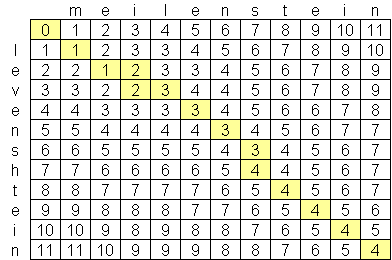
\includegraphics[width=0.68\textwidth]{Anexo1.png}
    \caption{Anexo distancia de Lvenshtein}
    \label{img:3}
\end{figure}

\section*{TFIDF }
En el proyecto de búsqueda de texto, se utilizan dos términos importantes: TF e IDF. El término TF (Term Frequency) se refiere a la relación entre la cantidad de veces que aparece una palabra en un documento específico (n) y la cantidad total de palabras en ese documento (N). Es decir, TF = n/N.

Por otro lado, el término IDF (Inverse Document Frequency) se refiere a la relación entre la cantidad total de documentos existentes (D) y la cantidad de documentos que contienen la palabra en cuestión (d), expresado como:
\begin{equation}
IDF = log(1 + \frac{D}{d})
\end{equation}

La combinación de estos dos términos permite calcular una puntuación de relevancia para cada palabra en cada documento, conocida como TF-IDF (Term Frequency-Inverse Document Frequency). Al multiplicar el valor de TF por el valor de IDF, se obtiene la relevancia de la palabra en el contexto del documento y del conjunto de todos los documentos.

En resumen, el cálculo de TF e IDF permite determinar la relevancia de una palabra en un conjunto de documentos, y la combinación de ambos valores mediante la fórmula TF-IDF permite obtener una puntuación de relevancia para cada palabra en cada documento.



\end{document}